\section{No observation choice is best everywhere}\label{sec:deploy}

\begin{figure}[t]
  \centering
  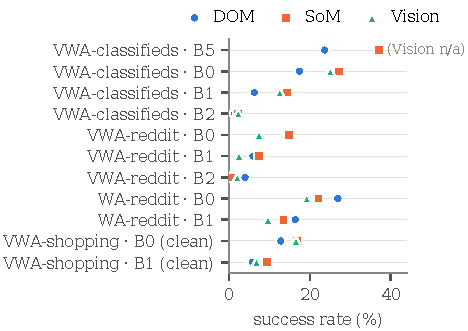
\includegraphics[width=\columnwidth]{fig_deploy}
  \caption{Success rate of the three deployment choices per cell. Shopping cells drop 46 state-sensitive tasks and every task the search-box defect touched in any mode (Appendix~\ref{app:harness}). B5's Vision run is excluded for a coordinate-contract defect.}
  % sources: routing_three_arm, routing_extension_cells
  \label{fig:deploy}
\end{figure}

The fused mode clearly leads text on classifieds (Figure~\ref{fig:deploy}). On reddit, text's leads all have intervals crossing zero once credit inherited from earlier episodes is removed. On classifieds the fused mode is the best of the three choices for B0 and B1, and beats DOM for GPT-5.6, whose Vision run is excluded. B2 solves too few tasks to order the modes. The margin over text is not small: \SoM$-$DOM is +9.82\pp\ [+3.57, +16.07] for B0 and +8.04\pp\ [+3.57, +12.95] for B1 (paired task bootstrap). % fusion_premium
On WA-reddit the order flips and text leads (\SoM$-$DOM $-4.81$\pp\ for B0 and $-2.88$\pp\ for B1, both intervals crossing zero). On VWA-reddit the weakest backbone does worse with the fused mode ($-2.96$\pp\ [$-5.91$, $-0.49$]). But three of its eight DOM successes were credited although their episodes never visited the target forum; an earlier episode had subscribed to it. Without them the gap is $-1.48$\pp\ [$-3.45$, $+0.49$] (Appendix~\ref{app:harness}). % fusion_premium, leakage_sensitivity
On shopping the fused mode is best or tied with Vision, on the filtered and on the full task sets (Figure~\ref{fig:deploy}, Table~\ref{tab:cells}).

Two cautions keep this descriptive. Cells on the same site share their tasks, so the eight are not eight independent replications. And there are four screenshot-free modes, not one. Comparing the best of four text variants with a single screenshot mode would introduce a selection effect, so we compare one mode per deployment choice, as practitioners do.

This section establishes only that the choice matters and depends on the workload. The rest of the paper asks whether the choice can be made per task.
